% Options for packages loaded elsewhere
\PassOptionsToPackage{unicode}{hyperref}
\PassOptionsToPackage{hyphens}{url}
%
\documentclass[
  ignorenonframetext,
]{beamer}
\usepackage{pgfpages}
\setbeamertemplate{caption}[numbered]
\setbeamertemplate{caption label separator}{: }
\setbeamercolor{caption name}{fg=normal text.fg}
\beamertemplatenavigationsymbolshorizontal
% Prevent slide breaks in the middle of a paragraph
\widowpenalties 1 10000
\raggedbottom
\setbeamertemplate{part page}{
  \centering
  \begin{beamercolorbox}[sep=16pt,center]{part title}
    \usebeamerfont{part title}\insertpart\par
  \end{beamercolorbox}
}
\setbeamertemplate{section page}{
  \centering
  \begin{beamercolorbox}[sep=12pt,center]{part title}
    \usebeamerfont{section title}\insertsection\par
  \end{beamercolorbox}
}
\setbeamertemplate{subsection page}{
  \centering
  \begin{beamercolorbox}[sep=8pt,center]{part title}
    \usebeamerfont{subsection title}\insertsubsection\par
  \end{beamercolorbox}
}
\AtBeginPart{
  \frame{\partpage}
}
\AtBeginSection{
  \ifbibliography
  \else
    \frame{\sectionpage}
  \fi
}
\AtBeginSubsection{
  \frame{\subsectionpage}
}

\usepackage{amsmath,amssymb}
\usepackage{lmodern}
\usepackage{iftex}
\ifPDFTeX
  \usepackage[T1]{fontenc}
  \usepackage[utf8]{inputenc}
  \usepackage{textcomp} % provide euro and other symbols
\else % if luatex or xetex
  \usepackage{unicode-math}
  \defaultfontfeatures{Scale=MatchLowercase}
  \defaultfontfeatures[\rmfamily]{Ligatures=TeX,Scale=1}
\fi
\usetheme[]{Madrid}
\usecolortheme{beaver}
% Use upquote if available, for straight quotes in verbatim environments
\IfFileExists{upquote.sty}{\usepackage{upquote}}{}
\IfFileExists{microtype.sty}{% use microtype if available
  \usepackage[]{microtype}
  \UseMicrotypeSet[protrusion]{basicmath} % disable protrusion for tt fonts
}{}
\makeatletter
\@ifundefined{KOMAClassName}{% if non-KOMA class
  \IfFileExists{parskip.sty}{%
    \usepackage{parskip}
  }{% else
    \setlength{\parindent}{0pt}
    \setlength{\parskip}{6pt plus 2pt minus 1pt}}
}{% if KOMA class
  \KOMAoptions{parskip=half}}
\makeatother
\usepackage{xcolor}
\newif\ifbibliography
\setlength{\emergencystretch}{3em} % prevent overfull lines
\setcounter{secnumdepth}{-\maxdimen} % remove section numbering

\usepackage{color}
\usepackage{fancyvrb}
\newcommand{\VerbBar}{|}
\newcommand{\VERB}{\Verb[commandchars=\\\{\}]}
\DefineVerbatimEnvironment{Highlighting}{Verbatim}{commandchars=\\\{\}}
% Add ',fontsize=\small' for more characters per line
\usepackage{framed}
\definecolor{shadecolor}{RGB}{241,243,245}
\newenvironment{Shaded}{\begin{snugshade}}{\end{snugshade}}
\newcommand{\AlertTok}[1]{\textcolor[rgb]{0.68,0.00,0.00}{#1}}
\newcommand{\AnnotationTok}[1]{\textcolor[rgb]{0.37,0.37,0.37}{#1}}
\newcommand{\AttributeTok}[1]{\textcolor[rgb]{0.40,0.45,0.13}{#1}}
\newcommand{\BaseNTok}[1]{\textcolor[rgb]{0.68,0.00,0.00}{#1}}
\newcommand{\BuiltInTok}[1]{\textcolor[rgb]{0.00,0.23,0.31}{#1}}
\newcommand{\CharTok}[1]{\textcolor[rgb]{0.13,0.47,0.30}{#1}}
\newcommand{\CommentTok}[1]{\textcolor[rgb]{0.37,0.37,0.37}{#1}}
\newcommand{\CommentVarTok}[1]{\textcolor[rgb]{0.37,0.37,0.37}{\textit{#1}}}
\newcommand{\ConstantTok}[1]{\textcolor[rgb]{0.56,0.35,0.01}{#1}}
\newcommand{\ControlFlowTok}[1]{\textcolor[rgb]{0.00,0.23,0.31}{#1}}
\newcommand{\DataTypeTok}[1]{\textcolor[rgb]{0.68,0.00,0.00}{#1}}
\newcommand{\DecValTok}[1]{\textcolor[rgb]{0.68,0.00,0.00}{#1}}
\newcommand{\DocumentationTok}[1]{\textcolor[rgb]{0.37,0.37,0.37}{\textit{#1}}}
\newcommand{\ErrorTok}[1]{\textcolor[rgb]{0.68,0.00,0.00}{#1}}
\newcommand{\ExtensionTok}[1]{\textcolor[rgb]{0.00,0.23,0.31}{#1}}
\newcommand{\FloatTok}[1]{\textcolor[rgb]{0.68,0.00,0.00}{#1}}
\newcommand{\FunctionTok}[1]{\textcolor[rgb]{0.28,0.35,0.67}{#1}}
\newcommand{\ImportTok}[1]{\textcolor[rgb]{0.00,0.46,0.62}{#1}}
\newcommand{\InformationTok}[1]{\textcolor[rgb]{0.37,0.37,0.37}{#1}}
\newcommand{\KeywordTok}[1]{\textcolor[rgb]{0.00,0.23,0.31}{#1}}
\newcommand{\NormalTok}[1]{\textcolor[rgb]{0.00,0.23,0.31}{#1}}
\newcommand{\OperatorTok}[1]{\textcolor[rgb]{0.37,0.37,0.37}{#1}}
\newcommand{\OtherTok}[1]{\textcolor[rgb]{0.00,0.23,0.31}{#1}}
\newcommand{\PreprocessorTok}[1]{\textcolor[rgb]{0.68,0.00,0.00}{#1}}
\newcommand{\RegionMarkerTok}[1]{\textcolor[rgb]{0.00,0.23,0.31}{#1}}
\newcommand{\SpecialCharTok}[1]{\textcolor[rgb]{0.37,0.37,0.37}{#1}}
\newcommand{\SpecialStringTok}[1]{\textcolor[rgb]{0.13,0.47,0.30}{#1}}
\newcommand{\StringTok}[1]{\textcolor[rgb]{0.13,0.47,0.30}{#1}}
\newcommand{\VariableTok}[1]{\textcolor[rgb]{0.07,0.07,0.07}{#1}}
\newcommand{\VerbatimStringTok}[1]{\textcolor[rgb]{0.13,0.47,0.30}{#1}}
\newcommand{\WarningTok}[1]{\textcolor[rgb]{0.37,0.37,0.37}{\textit{#1}}}

\providecommand{\tightlist}{%
  \setlength{\itemsep}{0pt}\setlength{\parskip}{0pt}}\usepackage{longtable,booktabs,array}
\usepackage{calc} % for calculating minipage widths
\usepackage{caption}
% Make caption package work with longtable
\makeatletter
\def\fnum@table{\tablename~\thetable}
\makeatother
\usepackage{graphicx}
\makeatletter
\def\maxwidth{\ifdim\Gin@nat@width>\linewidth\linewidth\else\Gin@nat@width\fi}
\def\maxheight{\ifdim\Gin@nat@height>\textheight\textheight\else\Gin@nat@height\fi}
\makeatother
% Scale images if necessary, so that they will not overflow the page
% margins by default, and it is still possible to overwrite the defaults
% using explicit options in \includegraphics[width, height, ...]{}
\setkeys{Gin}{width=\maxwidth,height=\maxheight,keepaspectratio}
% Set default figure placement to htbp
\makeatletter
\def\fps@figure{htbp}
\makeatother

\makeatletter
\@ifpackageloaded{tcolorbox}{}{\usepackage[many]{tcolorbox}}
\@ifpackageloaded{fontawesome5}{}{\usepackage{fontawesome5}}
\definecolor{quarto-callout-color}{HTML}{909090}
\definecolor{quarto-callout-note-color}{HTML}{0758E5}
\definecolor{quarto-callout-important-color}{HTML}{CC1914}
\definecolor{quarto-callout-warning-color}{HTML}{EB9113}
\definecolor{quarto-callout-tip-color}{HTML}{00A047}
\definecolor{quarto-callout-caution-color}{HTML}{FC5300}
\definecolor{quarto-callout-color-frame}{HTML}{acacac}
\definecolor{quarto-callout-note-color-frame}{HTML}{4582ec}
\definecolor{quarto-callout-important-color-frame}{HTML}{d9534f}
\definecolor{quarto-callout-warning-color-frame}{HTML}{f0ad4e}
\definecolor{quarto-callout-tip-color-frame}{HTML}{02b875}
\definecolor{quarto-callout-caution-color-frame}{HTML}{fd7e14}
\makeatother
\makeatletter
\makeatother
\makeatletter
\makeatother
\makeatletter
\@ifpackageloaded{caption}{}{\usepackage{caption}}
\AtBeginDocument{%
\ifdefined\contentsname
  \renewcommand*\contentsname{Table of contents}
\else
  \newcommand\contentsname{Table of contents}
\fi
\ifdefined\listfigurename
  \renewcommand*\listfigurename{List of Figures}
\else
  \newcommand\listfigurename{List of Figures}
\fi
\ifdefined\listtablename
  \renewcommand*\listtablename{List of Tables}
\else
  \newcommand\listtablename{List of Tables}
\fi
\ifdefined\figurename
  \renewcommand*\figurename{Figure}
\else
  \newcommand\figurename{Figure}
\fi
\ifdefined\tablename
  \renewcommand*\tablename{Table}
\else
  \newcommand\tablename{Table}
\fi
}
\@ifpackageloaded{float}{}{\usepackage{float}}
\floatstyle{ruled}
\@ifundefined{c@chapter}{\newfloat{codelisting}{h}{lop}}{\newfloat{codelisting}{h}{lop}[chapter]}
\floatname{codelisting}{Listing}
\newcommand*\listoflistings{\listof{codelisting}{List of Listings}}
\makeatother
\makeatletter
\@ifpackageloaded{caption}{}{\usepackage{caption}}
\@ifpackageloaded{subcaption}{}{\usepackage{subcaption}}
\makeatother
\makeatletter
\@ifpackageloaded{tcolorbox}{}{\usepackage[many]{tcolorbox}}
\makeatother
\makeatletter
\@ifundefined{shadecolor}{\definecolor{shadecolor}{rgb}{.97, .97, .97}}
\makeatother
\makeatletter
\makeatother
\ifLuaTeX
  \usepackage{selnolig}  % disable illegal ligatures
\fi
\IfFileExists{bookmark.sty}{\usepackage{bookmark}}{\usepackage{hyperref}}
\IfFileExists{xurl.sty}{\usepackage{xurl}}{} % add URL line breaks if available
\urlstyle{same} % disable monospaced font for URLs
\hypersetup{
  pdftitle={Uncertainty - Tidyverse 1},
  pdfauthor={Introduction to Quantitative Social Science},
  hidelinks,
  pdfcreator={LaTeX via pandoc}}

\title{Uncertainty - Tidyverse 1}
\subtitle{R data types and code style}
\author{Introduction to Quantitative Social Science}
\date{June 30, 2022}
\institute{Xiaolong Yang \and University of Tokyo}

\begin{document}
\frame{\titlepage}
\ifdefined\Shaded\renewenvironment{Shaded}{\begin{tcolorbox}[breakable, frame hidden, boxrule=0pt, enhanced, borderline west={3pt}{0pt}{shadecolor}, sharp corners, interior hidden]}{\end{tcolorbox}}\fi

\begin{frame}[fragile]{Today's Game Plan}
\protect\hypertarget{todays-game-plan}{}
\begin{enumerate}
\tightlist
\item
  data types: \textbf{vector}
\item
  code style
\item
  new functions in \textbf{Chapter 7: Uncertainty}
\end{enumerate}

\begin{itemize}
\tightlist
\item
  \texttt{geom\_pointrange()}
\item
  \texttt{facet\_grid()}
\end{itemize}

\begin{tcolorbox}[enhanced jigsaw, breakable, opacityback=0, toprule=.15mm, colframe=quarto-callout-note-color-frame, leftrule=.75mm, colback=white, arc=.35mm, rightrule=.15mm, bottomrule=.15mm, left=2mm]
\begin{minipage}[t]{5.5mm}
\textcolor{quarto-callout-note-color}{\faInfo}
\end{minipage}%
\begin{minipage}[t]{\textwidth - 5.5mm}
Today's in-class assignment: \texttt{china-women}\end{minipage}%
\end{tcolorbox}
\end{frame}

\hypertarget{data-types}{%
\section{Data types}\label{data-types}}

\begin{frame}{Visualizing Vectors: \emph{2 types of vector in R}}
\protect\hypertarget{visualizing-vectors-2-types-of-vector-in-r}{}
\begin{figure}

{\centering 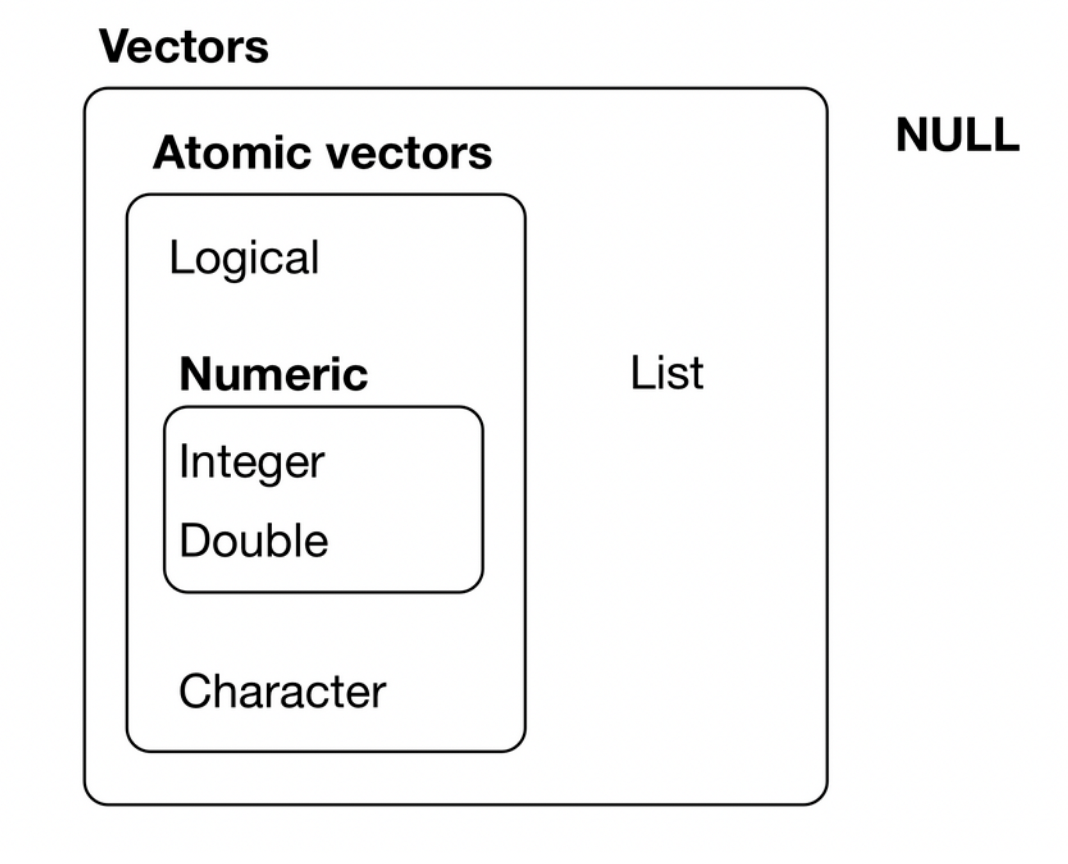
\includegraphics[width=0.5\textwidth,height=\textheight]{~/Desktop/vector.png}

}

\caption{The hierarchy of R's vector types; source: R4DS}

\end{figure}
\end{frame}

\begin{frame}[fragile]{Vectors: \emph{2 types of vector in R}}
\protect\hypertarget{vectors-2-types-of-vector-in-r}{}
\begin{columns}[c,totalwidth=8em]
\begin{column}{0.5\textwidth}
\textbf{Atomic Vector}

\begin{itemize}
\tightlist
\item
  Types

  \begin{itemize}
  \tightlist
  \item
    logical (TRUE/FALSE)
  \item
    numeric (integer, double)
  \item
    character
  \end{itemize}
\item
  \textbf{Homogeneous}: stores only one type of data
\item
  \texttt{typeof()} and \texttt{length()}
\end{itemize}

\begin{Shaded}
\begin{Highlighting}[]
\NormalTok{x }\OtherTok{\textless{}{-}} \FunctionTok{c}\NormalTok{(}\ConstantTok{TRUE}\NormalTok{, }\ConstantTok{TRUE}\NormalTok{, }\ConstantTok{FALSE}\NormalTok{)}

\FunctionTok{typeof}\NormalTok{(x)}
\end{Highlighting}
\end{Shaded}

\begin{verbatim}
[1] "logical"
\end{verbatim}

\begin{Shaded}
\begin{Highlighting}[]
\FunctionTok{length}\NormalTok{(x)}
\end{Highlighting}
\end{Shaded}

\begin{verbatim}
[1] 3
\end{verbatim}
\end{column}

\begin{column}{0.5\textwidth}
\textbf{List}

\begin{itemize}
\tightlist
\item
  \textbf{Heterogeneous}: stores different types of data
\end{itemize}

\begin{Shaded}
\begin{Highlighting}[]
\NormalTok{x }\OtherTok{\textless{}{-}} \FunctionTok{list}\NormalTok{(}\DecValTok{1}\NormalTok{, }
          \FunctionTok{c}\NormalTok{(}\DecValTok{2}\NormalTok{, }\DecValTok{3}\NormalTok{),}
          \StringTok{"QSS"}\NormalTok{,}
          \FunctionTok{list}\NormalTok{(}\DecValTok{4}\NormalTok{, }\DecValTok{5}\NormalTok{))}
          
\FunctionTok{str}\NormalTok{(x)}
\end{Highlighting}
\end{Shaded}

\begin{verbatim}
List of 4
 $ : num 1
 $ : num [1:2] 2 3
 $ : chr "QSS"
 $ :List of 2
  ..$ : num 4
  ..$ : num 5
\end{verbatim}
\end{column}
\end{columns}
\end{frame}

\begin{frame}{Visualizing Vectors: \emph{2 types of vector in R}}
\protect\hypertarget{visualizing-vectors-2-types-of-vector-in-r-1}{}
\begin{figure}

{\centering 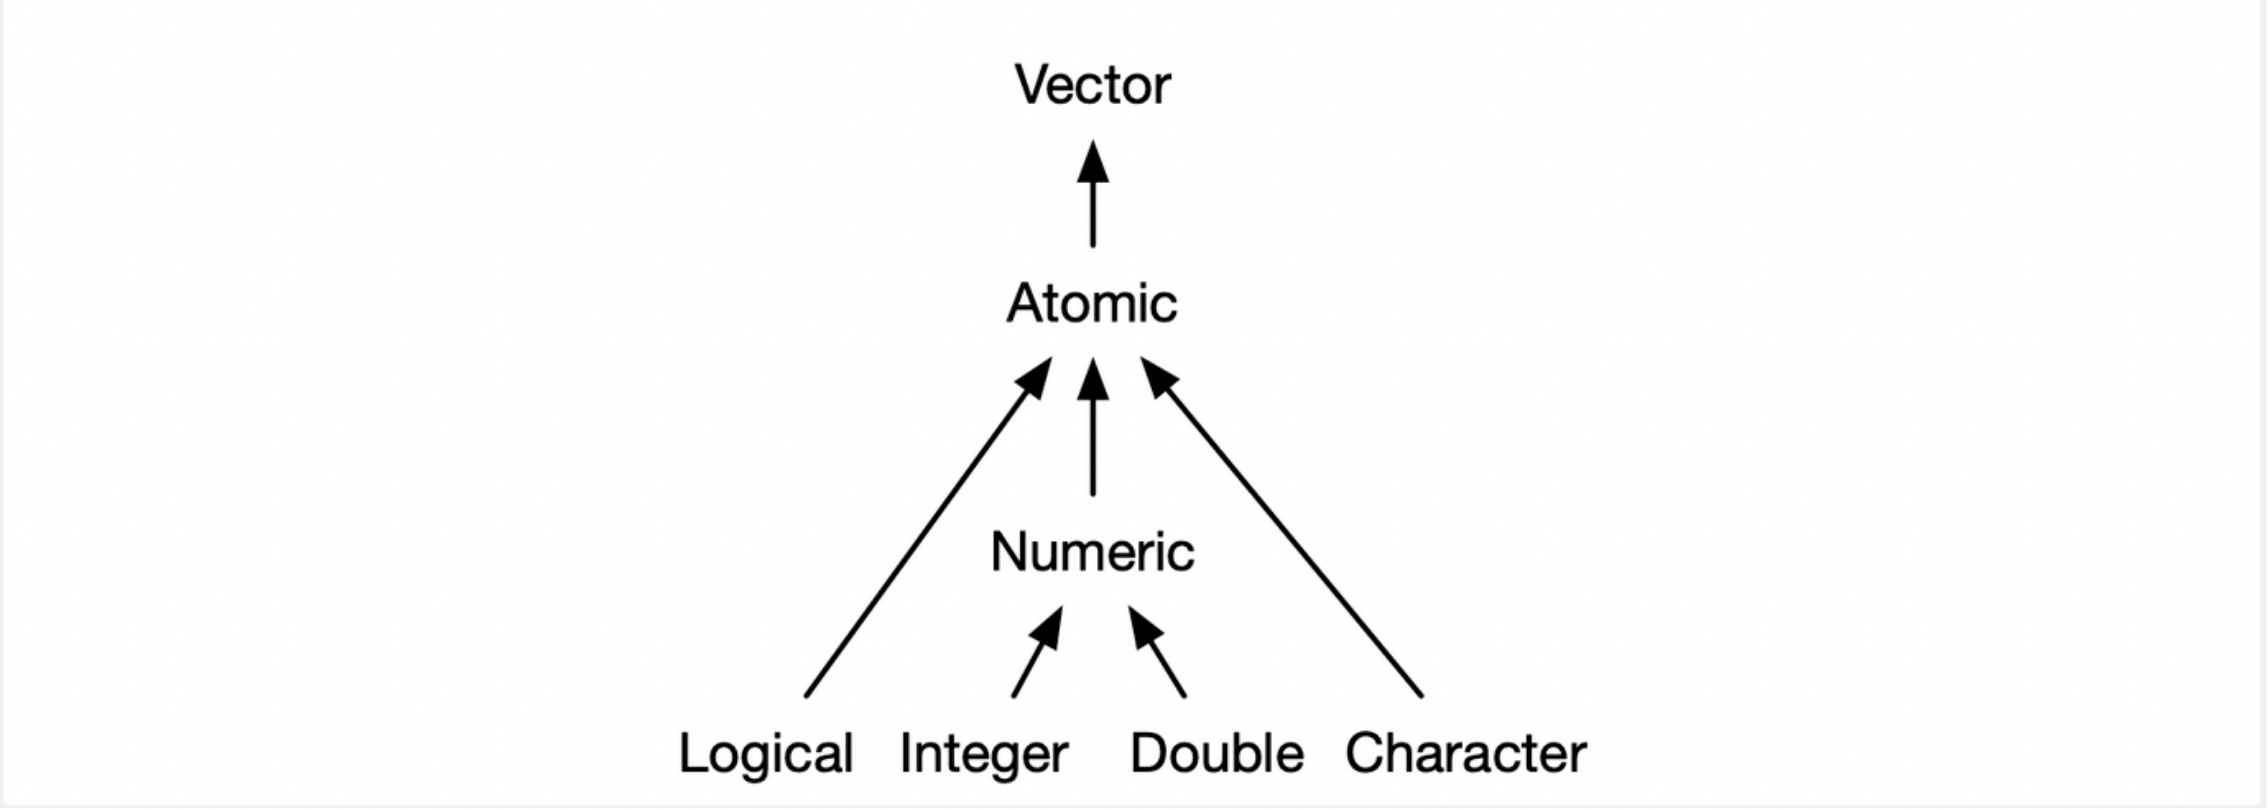
\includegraphics[width=1\textwidth,height=\textheight]{~/Desktop/atomic.png}

}

\caption{The hierarchy of Atomic vector; source: Advanced R}

\end{figure}
\end{frame}

\begin{frame}{Visualizing lists}
\protect\hypertarget{visualizing-lists}{}
\begin{figure}

{\centering 
\includegraphics[width=1\textwidth,height=\textheight]{~/Desktop/list.png}

}

\caption{Visualization of a list; source: Advanced R}

\end{figure}
\end{frame}

\begin{frame}[fragile]{Test functions}
\protect\hypertarget{test-functions}{}
\begin{itemize}
\tightlist
\item
  \texttt{in\_logical()}
\item
  \texttt{is\_integer()}
\item
  \texttt{is\_double()}
\item
  \texttt{is\_numeric()}
\item
  \texttt{is\_character()}
\item
  \texttt{is\_atomic()}
\item
  \texttt{is\_list()}
\item
  \texttt{is\_list()}
\end{itemize}

\begin{tcolorbox}[enhanced jigsaw, breakable, opacityback=0, toprule=.15mm, colframe=quarto-callout-tip-color-frame, leftrule=.75mm, colback=white, arc=.35mm, rightrule=.15mm, bottomrule=.15mm, left=2mm]
\begin{minipage}[t]{5.5mm}
\textcolor{quarto-callout-tip-color}{\faLightbulb}
\end{minipage}%
\begin{minipage}[t]{\textwidth - 5.5mm}
Good additional resources on R data types by Jenny Bryan
\href{https://jennybc.github.io/purrr-tutorial/bk00_vectors-and-lists.html}{\textbf{Vectors
and lists}} and \href{https://stat545.com/r-objects.html}{\textbf{R
objects and indexing}}\end{minipage}%
\end{tcolorbox}
\end{frame}

\begin{frame}{Data frames/tibbles}
\protect\hypertarget{data-framestibbles}{}
\begin{figure}

{\centering 
\includegraphics[width=1\textwidth,height=\textheight]{~/Desktop/tibble.png}

}

\caption{Visualization of data.frame and tibble as lists; source:
Advanced R}

\end{figure}
\end{frame}

\begin{frame}[fragile]{Data frames/tibbles}
\protect\hypertarget{data-framestibbles-1}{}
A data frame is a \textbf{named list}, but all the elements have the
same length

\begin{itemize}
\tightlist
\item
  elements in the list \texttt{=} columns
\item
  every column has the same length (number of observations)
\item
  \texttt{nth} row \texttt{=} \texttt{nth} items from each vector (nth
  observations)
\end{itemize}

\begin{Shaded}
\begin{Highlighting}[]
\FunctionTok{class}\NormalTok{(FLVoters)}
\end{Highlighting}
\end{Shaded}

\begin{verbatim}
[1] "data.frame"
\end{verbatim}

\begin{Shaded}
\begin{Highlighting}[]
\FunctionTok{typeof}\NormalTok{(FLVoters)}
\end{Highlighting}
\end{Shaded}

\begin{verbatim}
[1] "list"
\end{verbatim}

\begin{Shaded}
\begin{Highlighting}[]
\FunctionTok{length}\NormalTok{(FLVoters)}
\end{Highlighting}
\end{Shaded}

\begin{verbatim}
[1] 6
\end{verbatim}
\end{frame}

\begin{frame}
\begin{figure}

{\centering 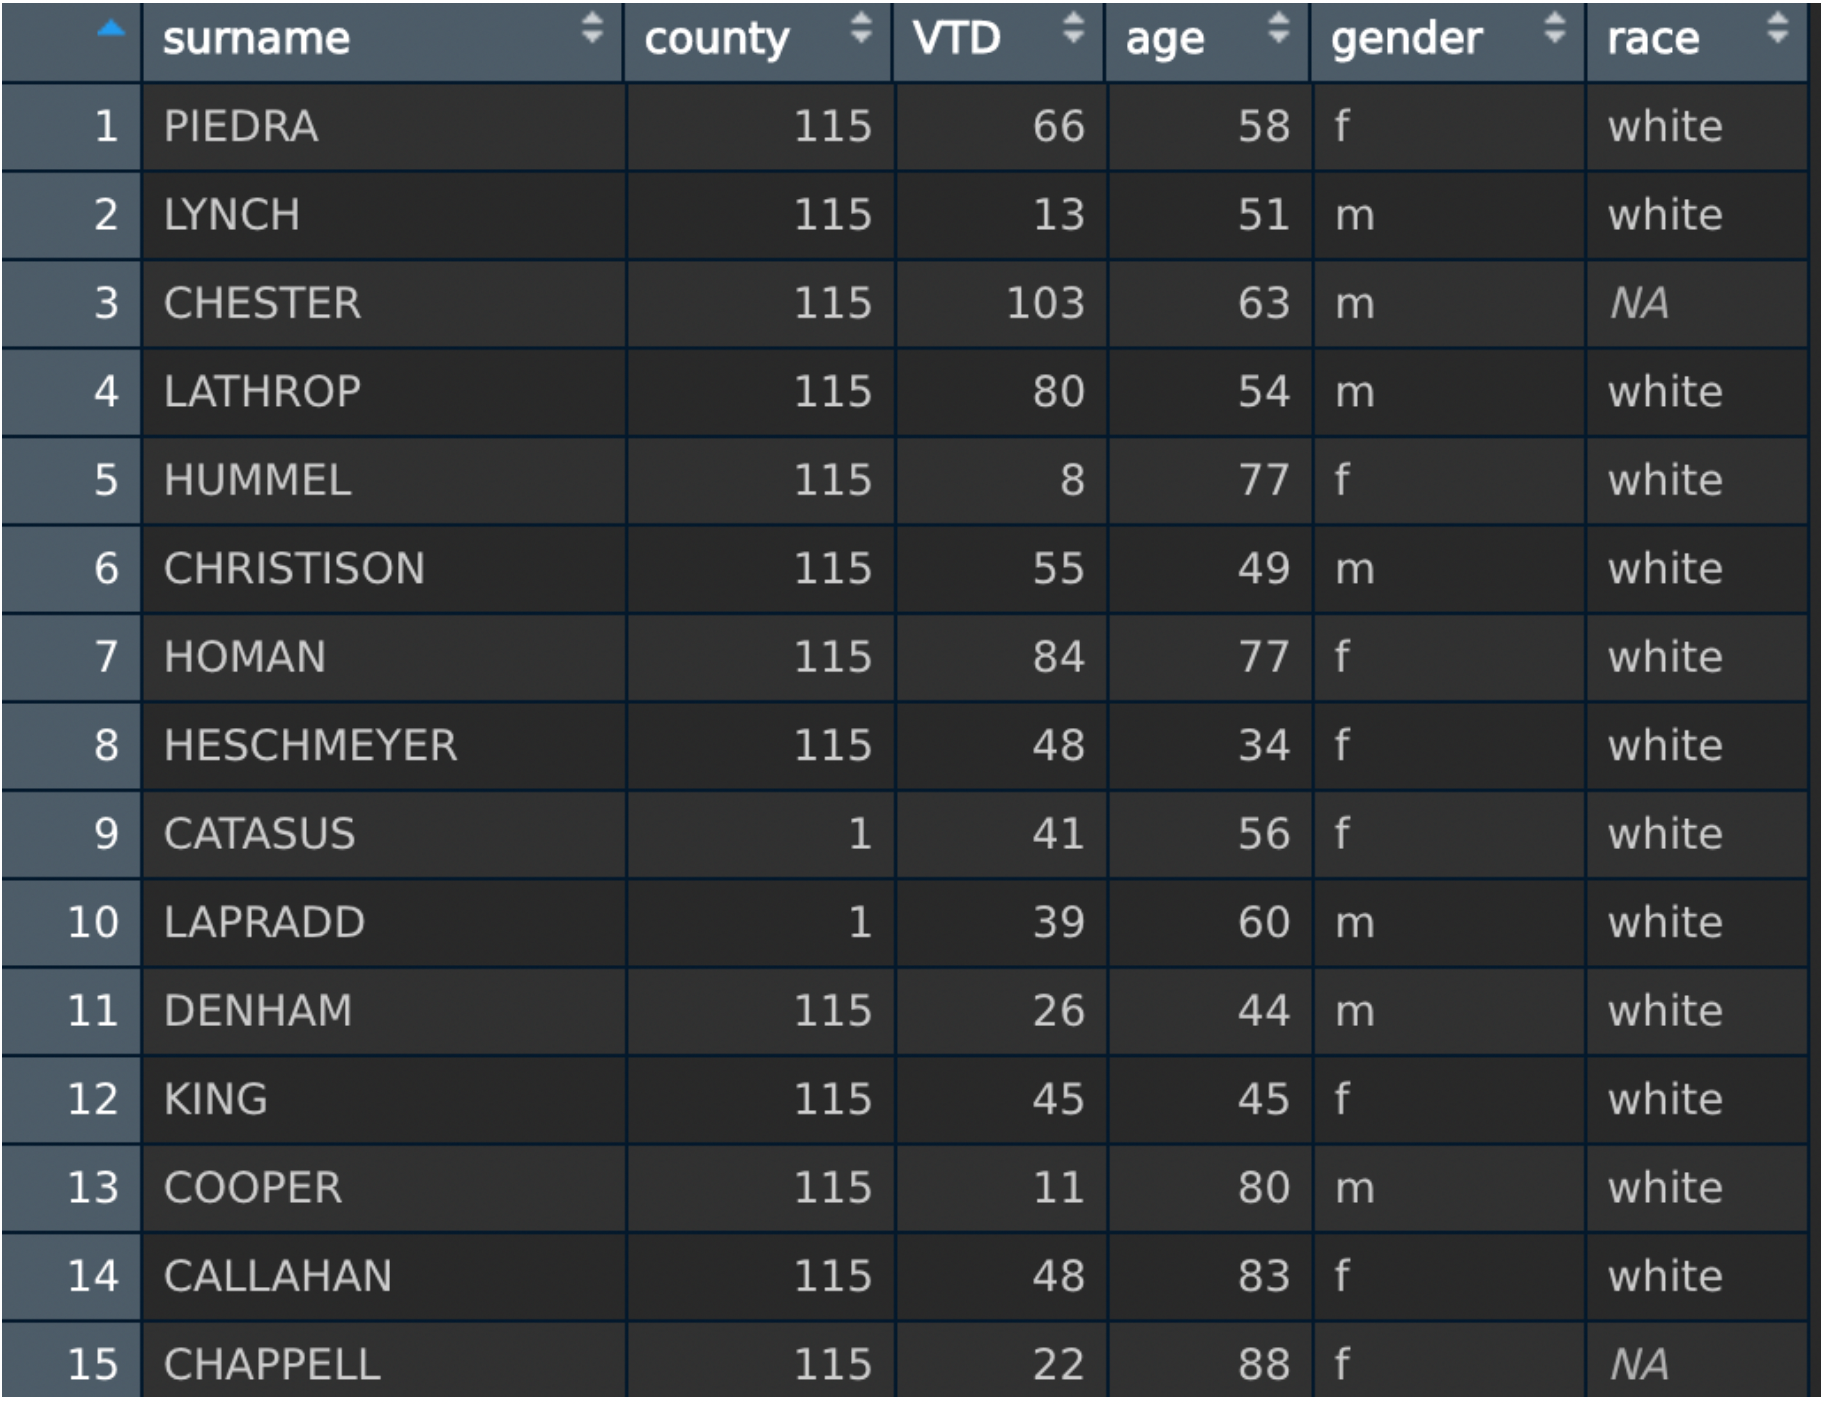
\includegraphics[width=0.8\textwidth,height=\textheight]{~/Desktop/FLVoters.png}

}

\caption{View FLVoters in RStudio}

\end{figure}
\end{frame}

\begin{frame}[fragile]{\texttt{purrr} \texttt{map()} function revisited}
\protect\hypertarget{purrr-map-function-revisited}{}
\begin{figure}

\begin{minipage}[t]{0.50\linewidth}

{\centering 

\raisebox{-\height}{

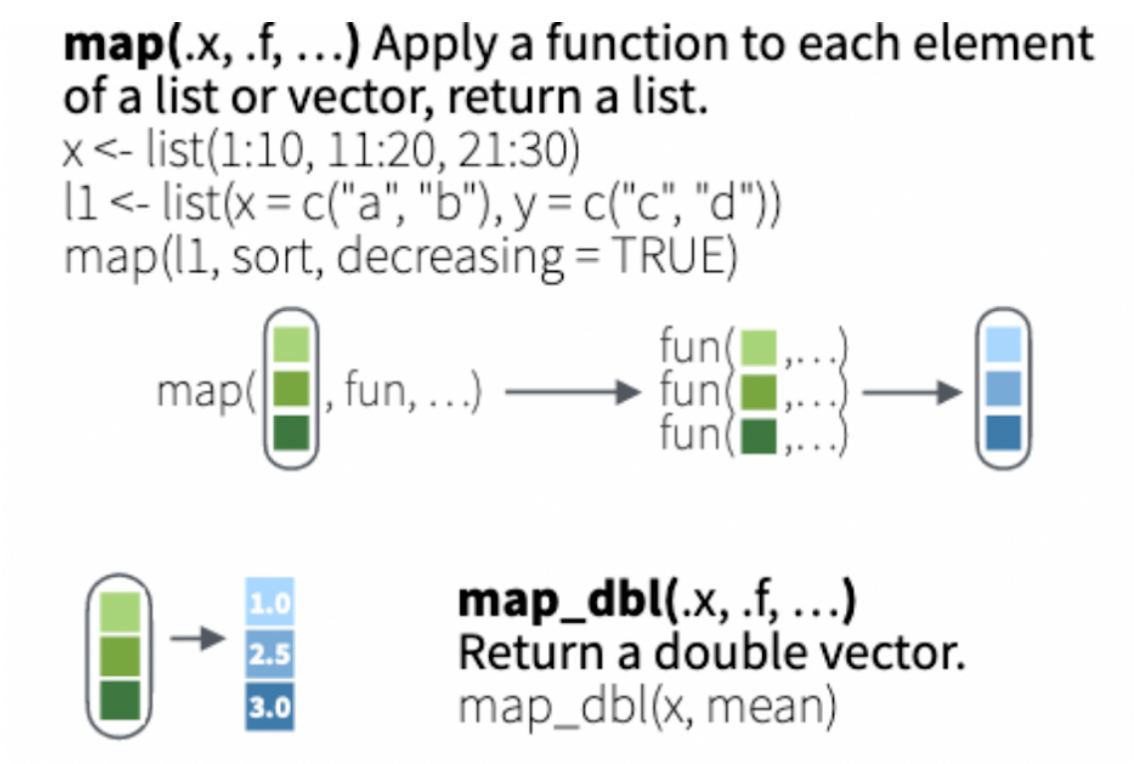
\includegraphics{~/Desktop/map1.png}

}

}

\end{minipage}%
%
\begin{minipage}[t]{0.50\linewidth}

{\centering 

\raisebox{-\height}{

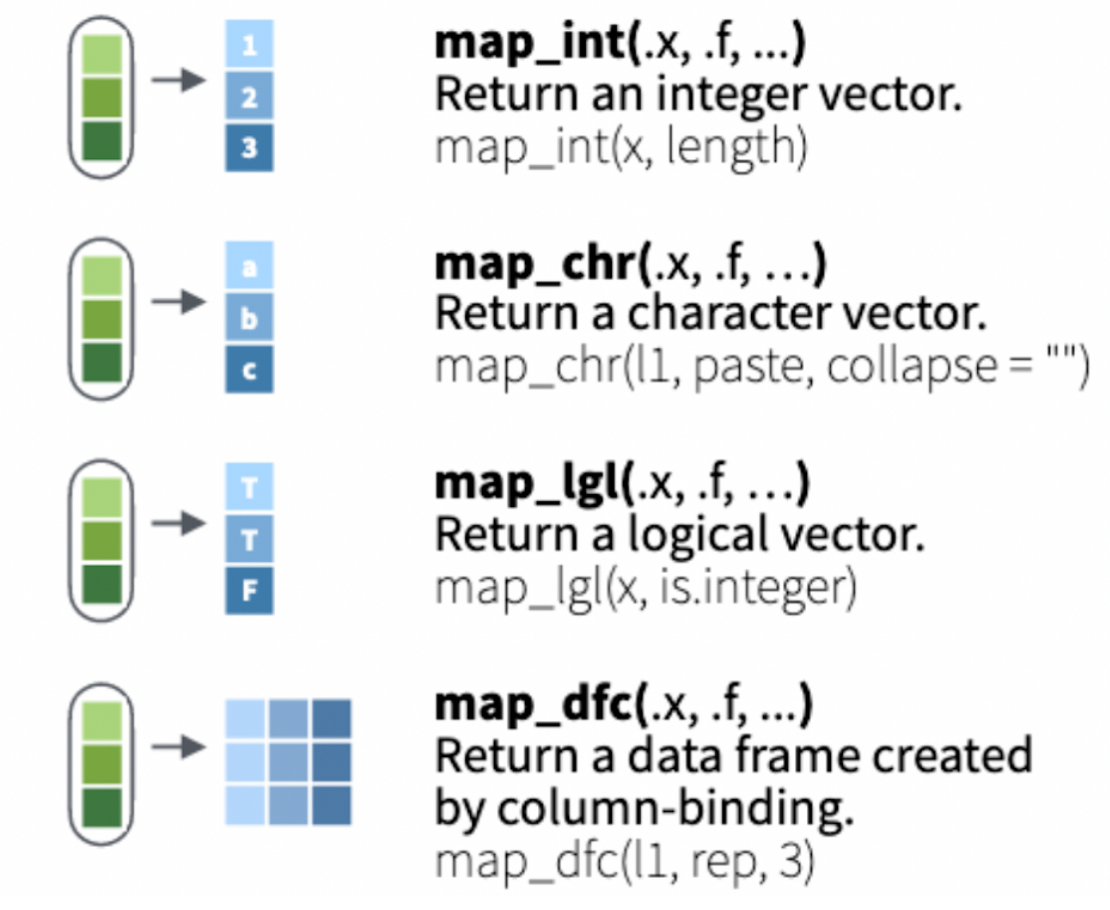
\includegraphics{~/Desktop/map2.png}

}

\caption{Source: \texttt{purrr} cheatsheet}

}

\end{minipage}%

\end{figure}
\end{frame}

\begin{frame}{Short summary: data structure in R}
\protect\hypertarget{short-summary-data-structure-in-r}{}
Vector as the most basic data type: workhorse of R

\begin{itemize}
\tightlist
\item
  atomic vector

  \begin{itemize}
  \tightlist
  \item
    \textbf{integer}, \textbf{double}, \textbf{character},
    \textbf{logical} (raw, complex)
  \item
    \textbf{homogeneous}
  \end{itemize}
\item
  list

  \begin{itemize}
  \tightlist
  \item
    a data frame/tibble as a list of equal-length elements
  \item
    \textbf{heterogeneous}
  \end{itemize}
\end{itemize}
\end{frame}

\hypertarget{code-style}{%
\section{Code style}\label{code-style}}

\begin{frame}[fragile]{Code style: syntax}
\protect\hypertarget{code-style-syntax}{}
\begin{itemize}
\tightlist
\item
  object names: snake\_case
\end{itemize}

\begin{Shaded}
\begin{Highlighting}[]
\CommentTok{\# Good}
\NormalTok{day\_one}
\NormalTok{day\_1}

\CommentTok{\# Bad}
\NormalTok{DayOne}
\NormalTok{dayone}
\end{Highlighting}
\end{Shaded}
\end{frame}

\begin{frame}[fragile]{Code style: syntax}
\protect\hypertarget{code-style-syntax-1}{}
\begin{itemize}
\tightlist
\item
  spacing: commas, parentheses
\end{itemize}

\begin{Shaded}
\begin{Highlighting}[]
\CommentTok{\# Good}
\NormalTok{x[, }\DecValTok{1}\NormalTok{]}
\FunctionTok{mean}\NormalTok{(x, }\AttributeTok{na.rm =} \ConstantTok{TRUE}\NormalTok{)}

\CommentTok{\# Bad}
\NormalTok{x[,}\DecValTok{1}\NormalTok{]}
\NormalTok{x[ ,}\DecValTok{1}\NormalTok{]}
\NormalTok{x[ , }\DecValTok{1}\NormalTok{]}
\FunctionTok{mean}\NormalTok{ (x, }\AttributeTok{na.rm =} \ConstantTok{TRUE}\NormalTok{)}
\FunctionTok{mean}\NormalTok{( x, }\AttributeTok{na.rm =} \ConstantTok{TRUE}\NormalTok{ )}
\end{Highlighting}
\end{Shaded}
\end{frame}

\begin{frame}[fragile]{Code style: syntax}
\protect\hypertarget{code-style-syntax-2}{}
\begin{itemize}
\tightlist
\item
  infix operators (\texttt{==}, \texttt{+}, \texttt{-},
  \texttt{\textless{}-}, etc.)
\end{itemize}

\begin{Shaded}
\begin{Highlighting}[]
\CommentTok{\# Good}
\NormalTok{height }\OtherTok{\textless{}{-}}\NormalTok{ (feet }\SpecialCharTok{*} \DecValTok{12}\NormalTok{) }\SpecialCharTok{+}\NormalTok{ inches}
\FunctionTok{mean}\NormalTok{(x, }\AttributeTok{na.rm =} \ConstantTok{TRUE}\NormalTok{)}

\CommentTok{\# Bad}
\NormalTok{height}\OtherTok{\textless{}{-}}\NormalTok{feet}\SpecialCharTok{*}\DecValTok{12}\SpecialCharTok{+}\NormalTok{inches}
\FunctionTok{mean}\NormalTok{(x, }\AttributeTok{na.rm=}\ConstantTok{TRUE}\NormalTok{)}
\end{Highlighting}
\end{Shaded}
\end{frame}

\begin{frame}[fragile]{Code style: syntax}
\protect\hypertarget{code-style-syntax-3}{}
\begin{itemize}
\tightlist
\item
  long lines: 80 characters per line

  \begin{itemize}
  \tightlist
  \item
    use one line each for the function name, each argument, and the
    closing
  \end{itemize}
\end{itemize}

\begin{Shaded}
\begin{Highlighting}[]
\CommentTok{\# Good}
\FunctionTok{do\_something\_very\_complicated}\NormalTok{(}
  \AttributeTok{something =} \StringTok{"that"}\NormalTok{,}
  \AttributeTok{requires =}\NormalTok{ many,}
  \AttributeTok{arguments =} \StringTok{"some of which may be long"}
\NormalTok{)}

\CommentTok{\# Bad}
\FunctionTok{do\_something\_very\_complicated}\NormalTok{(}\StringTok{"that"}\NormalTok{, requires, many, arguments,}
                              \StringTok{"some of which may be long"}
\NormalTok{                              )}
\end{Highlighting}
\end{Shaded}
\end{frame}

\begin{frame}[fragile]{Code style: syntax}
\protect\hypertarget{code-style-syntax-4}{}
\begin{itemize}
\tightlist
\item
  assignment
\end{itemize}

\begin{Shaded}
\begin{Highlighting}[]
\CommentTok{\# Good}
\NormalTok{x }\OtherTok{\textless{}{-}} \DecValTok{5}

\CommentTok{\# Bad}
\NormalTok{x }\OtherTok{=} \DecValTok{5}
\end{Highlighting}
\end{Shaded}
\end{frame}

\begin{frame}[fragile]{Code style: syntax}
\protect\hypertarget{code-style-syntax-5}{}
\begin{itemize}
\tightlist
\item
  logical vectors
\end{itemize}

\begin{Shaded}
\begin{Highlighting}[]
\CommentTok{\# Good}
\NormalTok{na.rm }\OtherTok{=} \ConstantTok{TRUE}
\NormalTok{na.rm }\OtherTok{=} \ConstantTok{FALSE}

\CommentTok{\# Bad}
\NormalTok{na.rm }\OtherTok{=}\NormalTok{ T}
\NormalTok{na.rm }\OtherTok{=}\NormalTok{ F}
\end{Highlighting}
\end{Shaded}
\end{frame}

\begin{frame}[fragile]{Code style: syntax}
\protect\hypertarget{code-style-syntax-6}{}
\begin{itemize}
\tightlist
\item
  quotation marks
\end{itemize}

\begin{Shaded}
\begin{Highlighting}[]
\CommentTok{\# Good}
\StringTok{"Text"}
\StringTok{\textquotesingle{}Text with "quotes"\textquotesingle{}}

\CommentTok{\# Bad}
\StringTok{\textquotesingle{}Text\textquotesingle{}}
\StringTok{\textquotesingle{}Text with "double" and }\SpecialCharTok{\textbackslash{}\textquotesingle{}}\StringTok{single}\SpecialCharTok{\textbackslash{}\textquotesingle{}}\StringTok{ quotes\textquotesingle{}}
\end{Highlighting}
\end{Shaded}
\end{frame}

\begin{frame}[fragile]{Code style: syntax}
\protect\hypertarget{code-style-syntax-7}{}
\begin{itemize}
\tightlist
\item
  comments: each line of a comment begins with \texttt{\#} and a single
  space
\end{itemize}

\begin{Shaded}
\begin{Highlighting}[]
\CommentTok{\# regress y on x}
\NormalTok{fit }\OtherTok{\textless{}{-}} \FunctionTok{lm}\NormalTok{(y }\SpecialCharTok{\textasciitilde{}}\NormalTok{ x, }\AttributeTok{data =}\NormalTok{ df) }\CommentTok{\# why lm()}
\end{Highlighting}
\end{Shaded}
\end{frame}

\begin{frame}{Code style guides}
\protect\hypertarget{code-style-guides}{}
\begin{tcolorbox}[enhanced jigsaw, titlerule=0mm, left=2mm, toptitle=1mm, leftrule=.75mm, coltitle=black, rightrule=.15mm, bottomrule=.15mm, breakable, opacityback=0, toprule=.15mm, colframe=quarto-callout-note-color-frame, opacitybacktitle=0.6, arc=.35mm, colbacktitle=quarto-callout-note-color!10!white, bottomtitle=1mm, title=\textcolor{quarto-callout-note-color}{\faInfo}\hspace{0.5em}{Note}, colback=white]

\begin{itemize}
\tightlist
\item
  \href{https://google.github.io/styleguide/Rguide.html}{\textbf{Google's
  R Style Guide}}
\item
  \href{https://style.tidyverse.org/index.html}{\textbf{The Tidyverse
  Style Guide}}
\item
  \href{https://cs50.harvard.edu/ap/2020/assets/pdfs/pseudocode.pdf}{\textbf{Computer
  Programming: Pseudocode by Harvard CS50}}
\end{itemize}

\end{tcolorbox}
\end{frame}

\hypertarget{new-functions-in-chapter-7-uncertainty}{%
\section{\texorpdfstring{New functions in \textbf{Chapter 7:
Uncertainty}}{New functions in Chapter 7: Uncertainty}}\label{new-functions-in-chapter-7-uncertainty}}

\begin{frame}[fragile]{\texttt{ggplot}: \texttt{geom\_pointrange()}}
\protect\hypertarget{ggplot-geom_pointrange}{}
\begin{itemize}
\tightlist
\item
  draws points that shows a vertical interval defined by \texttt{x},
  \texttt{ymin} and \texttt{ymax}

  \begin{itemize}
  \tightlist
  \item
    the 95\% confidence intervals
  \end{itemize}
\end{itemize}

\begin{Shaded}
\begin{Highlighting}[]
\FunctionTok{ggplot}\NormalTok{(poll\_pred, }\FunctionTok{aes}\NormalTok{(actual, Obama)) }\SpecialCharTok{+}
  \FunctionTok{geom\_abline}\NormalTok{(}\AttributeTok{intercept =} \DecValTok{0}\NormalTok{,}
              \AttributeTok{slope =} \DecValTok{1}\NormalTok{) }\SpecialCharTok{+}
  \FunctionTok{geom\_pointrange}\NormalTok{(}\FunctionTok{aes}\NormalTok{(}\AttributeTok{ymin =}\NormalTok{ ci\_lower,}
                      \AttributeTok{ymax =}\NormalTok{ ci\_upr)) }\SpecialCharTok{+}
\NormalTok{  ...}
\end{Highlighting}
\end{Shaded}
\end{frame}

\begin{frame}[fragile]{\texttt{ggplot}: \texttt{geom\_pointrange()}}
\protect\hypertarget{ggplot-geom_pointrange-1}{}
\begin{itemize}
\tightlist
\item
  draws points that show a vertical interval defined by \texttt{x},
  \texttt{ymin} and \texttt{ymax}

  \begin{itemize}
  \tightlist
  \item
    the 95\% confidence intervals
    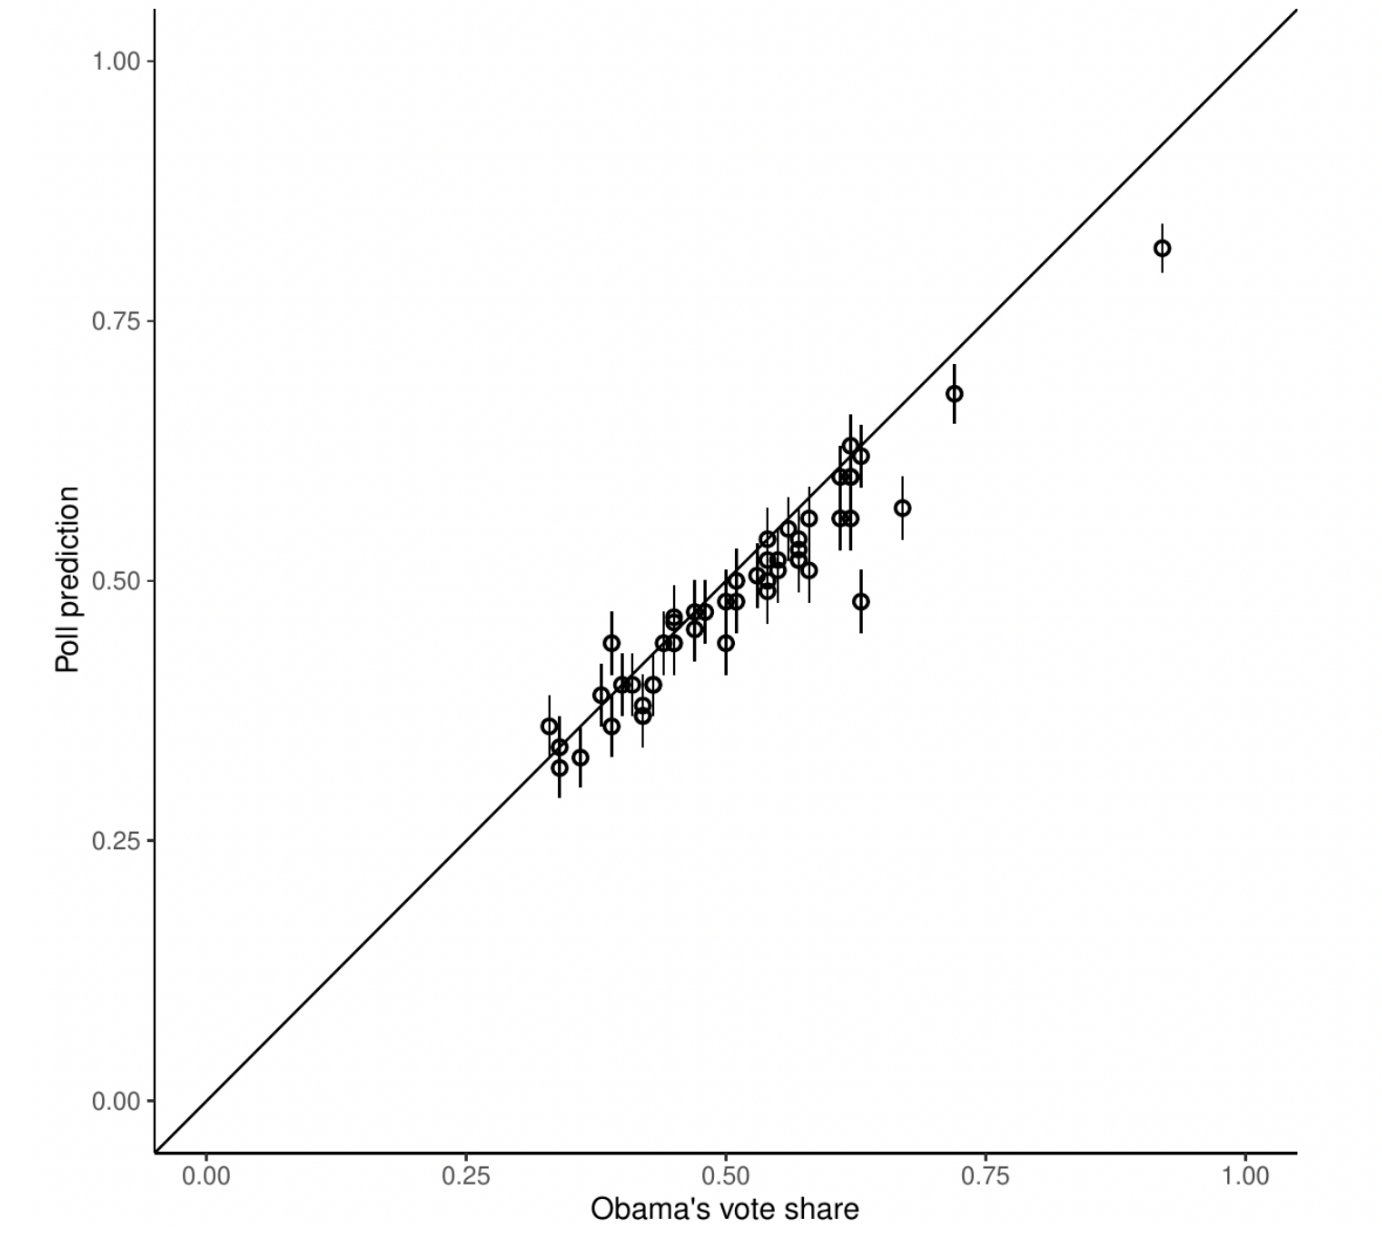
\includegraphics[width=0.6\textwidth,height=\textheight]{~/Desktop/ci.png}
  \end{itemize}
\end{itemize}
\end{frame}

\begin{frame}[fragile]{\texttt{ggplot}: \texttt{facet\_grid()}}
\protect\hypertarget{ggplot-facet_grid}{}
\begin{itemize}
\tightlist
\item
  Create separate panels for different class types defined by row and
  column faceting variables
\item
  facet\_grid(. \textasciitilde{} y)

  \begin{itemize}
  \tightlist
  \item
    spreads \texttt{y} across columns \(\rightarrow\) comparison of
    \texttt{y} positions
  \end{itemize}
\end{itemize}

\begin{Shaded}
\begin{Highlighting}[]
\NormalTok{base }\OtherTok{\textless{}{-}}\NormalTok{ FLVoters }\SpecialCharTok{\%\textgreater{}\%} 
  \FunctionTok{na.omit}\NormalTok{() }\SpecialCharTok{\%\textgreater{}\%} 
  \FunctionTok{ggplot}\NormalTok{(}\FunctionTok{aes}\NormalTok{(age, VTD)) }\SpecialCharTok{+}
  \FunctionTok{geom\_point}\NormalTok{()}

\NormalTok{base }\SpecialCharTok{+}
  \FunctionTok{facet\_grid}\NormalTok{(. }\SpecialCharTok{\textasciitilde{}}\NormalTok{ gender)}
\end{Highlighting}
\end{Shaded}
\end{frame}

\begin{frame}
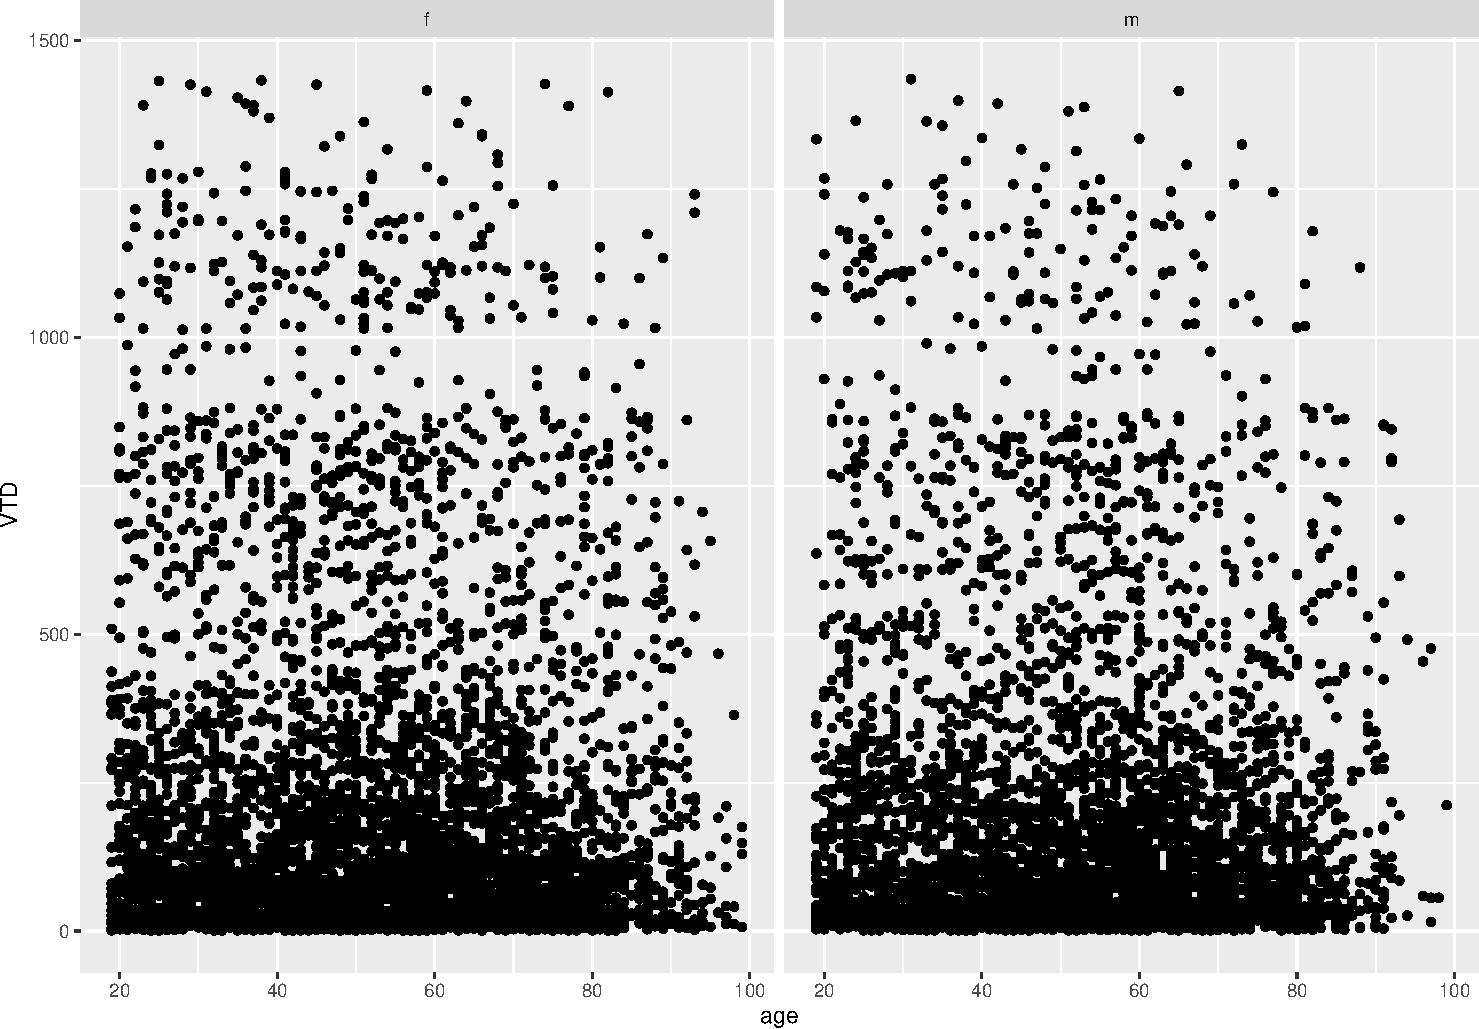
\includegraphics{uncertainty-tidy-1_files/figure-beamer/unnamed-chunk-15-1.pdf}
\end{frame}

\begin{frame}[fragile]{\texttt{ggplot}: \texttt{facet\_grid()}}
\protect\hypertarget{ggplot-facet_grid-1}{}
\begin{itemize}
\tightlist
\item
  Create separate panels for different class types defined by row and
  column faceting variables
\item
  facet\_grid(x \textasciitilde{} .)

  \begin{itemize}
  \tightlist
  \item
    spreads \texttt{x} across rows \(\rightarrow\) comparison of
    \texttt{x} positions
  \end{itemize}
\end{itemize}

\begin{Shaded}
\begin{Highlighting}[]
\NormalTok{base }\SpecialCharTok{+}
  \FunctionTok{facet\_grid}\NormalTok{(race }\SpecialCharTok{\textasciitilde{}}\NormalTok{ .)}
\end{Highlighting}
\end{Shaded}
\end{frame}

\begin{frame}
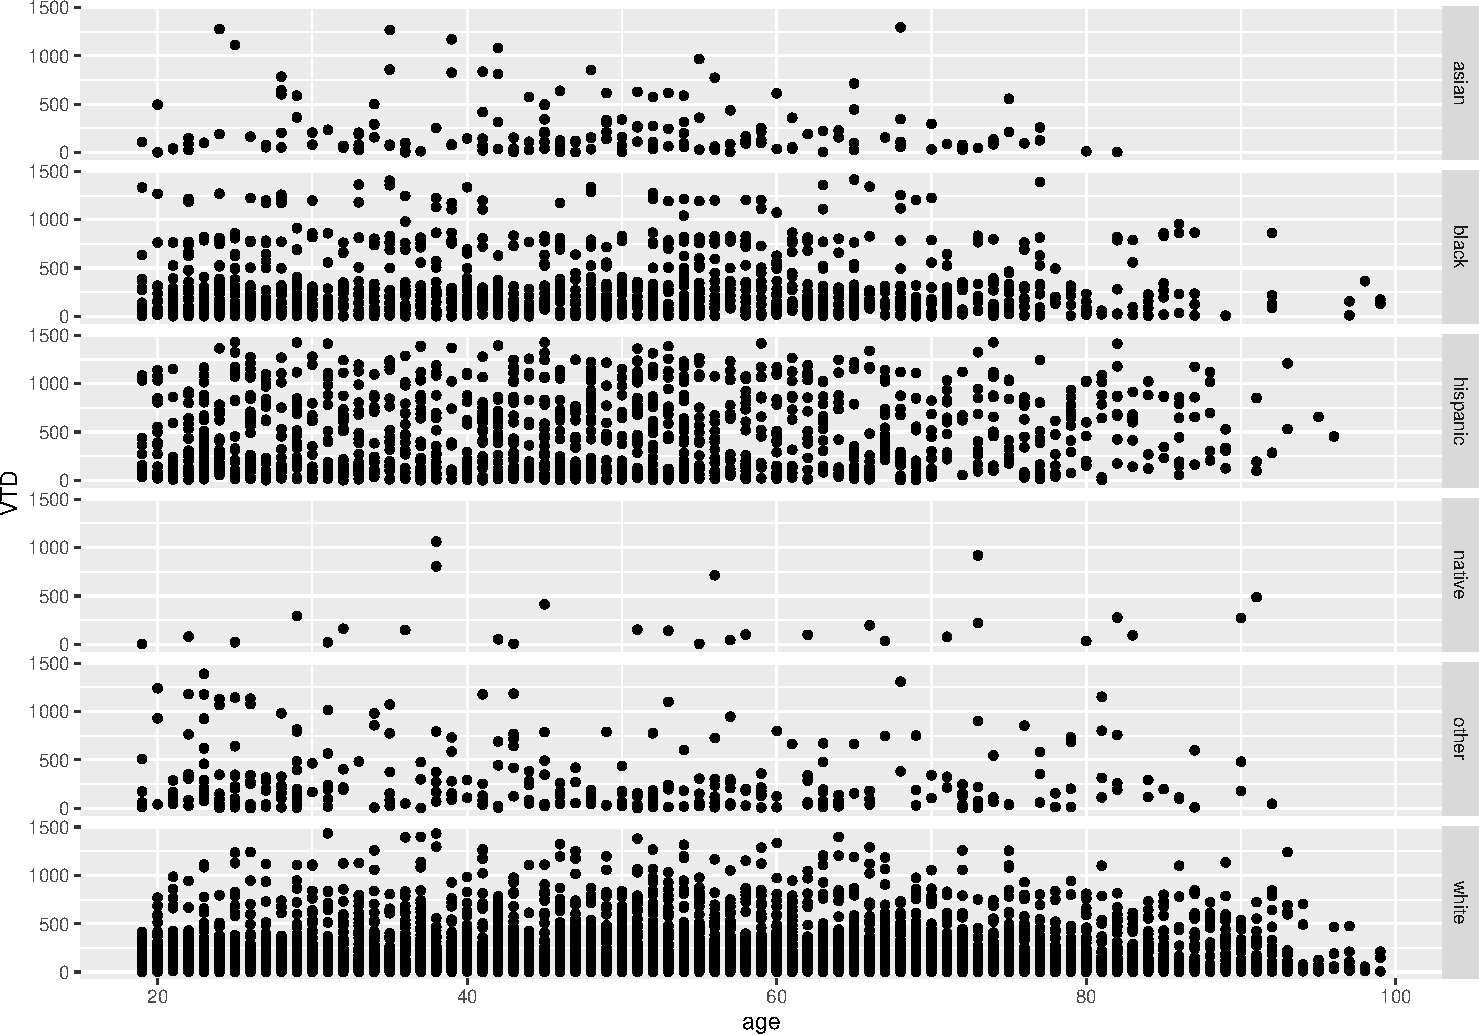
\includegraphics{uncertainty-tidy-1_files/figure-beamer/unnamed-chunk-17-1.pdf}
\end{frame}

\begin{frame}[fragile]{\texttt{ggplot}: \texttt{facet\_grid()}}
\protect\hypertarget{ggplot-facet_grid-2}{}
\begin{itemize}
\tightlist
\item
  Create separate panels for different class types defined by row and
  column faceting variables
\item
  \texttt{facet\_grid(x\ \textasciitilde{}\ y)}
\end{itemize}

\begin{Shaded}
\begin{Highlighting}[]
\NormalTok{base }\SpecialCharTok{+}
  \FunctionTok{facet\_grid}\NormalTok{(race }\SpecialCharTok{\textasciitilde{}}\NormalTok{ gender)}
\end{Highlighting}
\end{Shaded}
\end{frame}

\begin{frame}
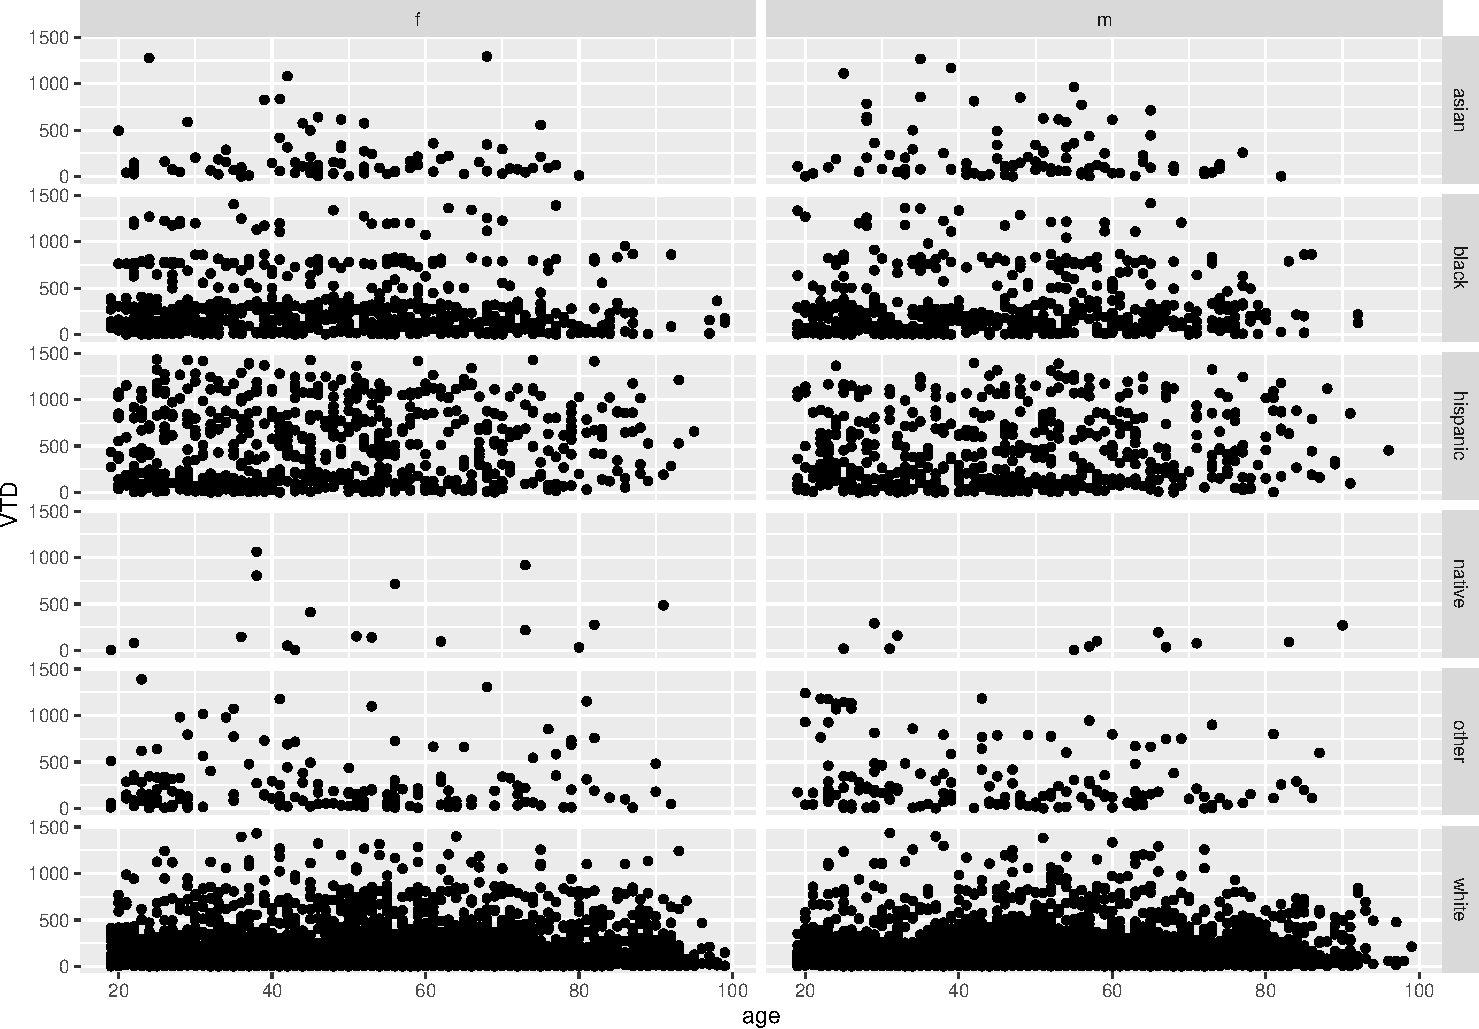
\includegraphics{uncertainty-tidy-1_files/figure-beamer/unnamed-chunk-19-1.pdf}
\end{frame}

\begin{frame}[fragile]{\textbf{What we learnt}}
\protect\hypertarget{what-we-learnt}{}
\begin{itemize}
\tightlist
\item
  data types: \textbf{vector}
\item
  code style
\item
  new \texttt{ggplot} functions
\end{itemize}
\end{frame}

\begin{frame}{Future Game Plan}
\protect\hypertarget{future-game-plan}{}
\begin{itemize}
\tightlist
\item
  reducing duplication: \textbf{iteration}
\item
  new functions in \textbf{chapter 7: Uncertainty (7.2, 7.3)}
\end{itemize}
\end{frame}



\end{document}
